\documentclass{article}

\usepackage{graphicx}

\title{Develop a Better Understanding of the Factors Involved With Facilitating the Movement of Refugees From Their Countries of Origin Into Safe Haven Countries}
\author{Jacob Denson}

\begin{document}

\maketitle

This problem breaks down into multiple problems.

\begin{enumerate}
    \item {\bf What are the factors involved with moving refugees?}

    What attributes enable or inhibit the safe and efficient movement of refugees. As an example, the individuals (plus resources the individuals have), routes, types of transportation, country capacity (plus entry points). The UN asks us to prioritize the health and safety of refugees.

    \item {\bf How do we gain a better understanding of the factors?}

    Create a model of optimal refugee movement, considering accessibility of transport, safety of route, and resource capacities of countries. Use metrics considered to predict the number of refugees that are to be moved, as well as the rate and point of entry necessary to accomodate their movement. Explain new elements you have incorporated into the migration process.

    It should be noted that we must account for dynamically changing environmental factors. Our model should exhibit a use of endogenous change (prepositioning and allocating resources) to form the best route planning approach. Exogenous parameters (unavoidable, unpredictable events, like the terrorist attack in France) must also be considered.

    \item {\bf Propose a set of policies to the UN}

    Write a report to the UN, proposing a set of policies to enact which will support the conditions for optimal migration (optimal to the UN's views).
\end{enumerate}

The 1951 refugee convention defines a refugee to be ``owing to a well-founded fear of being persecuted for reasons of race, religion, nationality, membership of a particular social group or political opinion, is outside the country of his nationality, and is unable to, or owing to such fear, is unwilling to avail himself of the protection of that country''\footnote{http://www.unhcr.org/pages/49da0e466.html}, rather than a migrant, who is just someone moving from one country to another.

Immigrants travel multiple routes -- beginning at the middle east, and travelling through the West, East, and Central Mediterranean, the West Balkans, the Eastern Borders, and from Albania to Greece.

\begin{center}
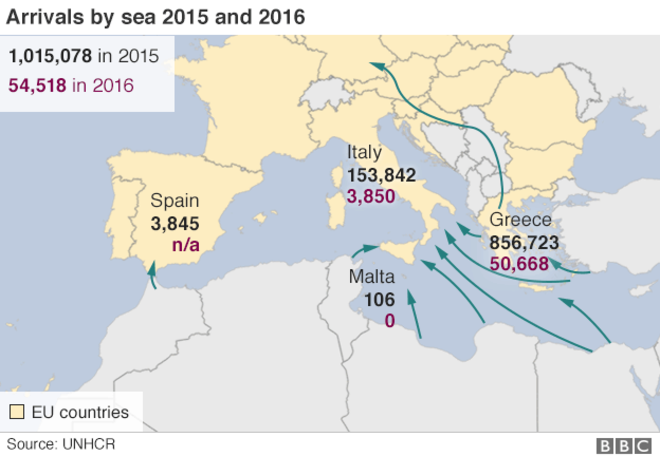
\includegraphics[scale=0.5]{travelmap}
\end{center}

\begin{enumerate}
    \item The majority of refugees resettle in the middle eastern countries of Jordan, Lebanon, and Turkey.
    \item 1,015,078 refugees arrived by sea in 2015.
    \item 942,000 refugees sought asylum in the European Union in 2015\footnote{Eurostat}.
    \item 315,000 have sought asylum in Germany, yet more than 1 million have been counted in Germany's EASY system\footnote{http://www.bbc.com/news/world-europe-34131911}.
    \item 174,055 applied in Hungary.
\end{enumerate}

Illegal immigration is dangerous, both for political relationships ensuring sustained immigration, and the danger to the immigrants of crossing the border.

\begin{enumerate}
    \item Poorly managed camps in Hungary damaged migrants reputation, leading to a surge in the popularity of the radical nationalist Jobbik party\footnote{http://www.bbc.com/news/world-europe-34280460}. It is difficult to control the way countries will handle the immigration crises, so this is an exogenous factor.
    \item In other countries, such as Germany, strong moral foundations protect the influx of immigration\footnote{http://www.bbc.com/news/world-europe-33700624}, with little (and strongly opposed) backlash at the new immigration policies.
    \item The Paris attacks threatened relations about refugees. A Polish minister stated that ``we were too idealistic'' \footnote{http://www.bbc.com/news/world-europe-34826438}. The attack deepened the level of insecurity across Europe, since it was believed that the terrorists snuck into the country with refugees. Regardless of the truth of these facts (the leader was Belgian), the coinciding events were treated as such, and has lead to border problems in the country.
\end{enumerate}

The difference in each country's utility to hold refugees is integral to how important it is to uphold their immigration policy.

Economically, immigration should be beneficial to host countries. A well defined immigration policy, distributed across the continent, should not be a problem

\begin{enumerate}
    \item Our best evidence suggests that immigration is usually economically beneficial for host countries. The majority of refugees arriving on European shores are able-bodied and unlikely to be an exception to this general rule. So the best way for Europe to help would be to offer immediate legal residency and access to labour markets. It might be politically expedient to restrict access to some welfare benefits but most migrants will be keen to work regardless. \footnote{http://www.telegraph.co.uk/news/worldnews/europe/11845205/Why-do-refugees-and-migrants-come-to-Europe-and-what-must-be-done-to-ease-the-crisis.html}
\end{enumerate}

Note that our proposal is a short term proposal. The only way to permanantly ease the migrant situation in Europe is to end the conflicts that make people flee their countries in the first place. Therefore, we should only project our models into short time periods in the future (5 years?).

How much do refugees move once they enter countries? Evidence to suggest immigrants attempt to flee Hungary and enter Germany.

Things to research for tomorrow:
\begin{enumerate}
    \item History, pertaining to dangers and effects of certain decisions on immigration policy.
    \item The UN's framework and objectives for the goals of refugee immigration.
    \item How NGOs fit into the immigration picture.
    \item How much does immigration cost?
    \item Justification for having a temporary solution vs a permanant solution.
    \item Look up the application for official refugee status.
    \item How many immigrants do we need to accomodate?
    \item What Routes do immigrants take - what type of transportation are they taking?
    \item Where are immigrants trying to go?
    \item Quotas for countries.
    \item Legal routes for immigrants immigrate.
\end{enumerate}

\end{document}